\documentclass[../main/NEMO_manual]{subfiles}

\begin{document}

\chapter{Lateral Ocean Physics (LDF)}
\label{chap:LDF}

\thispagestyle{plain}

\chaptertoc

\paragraph{Changes record} ~\\

{\footnotesize
  \begin{tabularx}{\textwidth}{l||X|X}
    Release & Author(s) & Modifications \\
    \hline
    {\em   4.0} & {\em ...} & {\em ...} \\
    {\em   3.6} & {\em ...} & {\em ...} \\
    {\em   3.4} & {\em ...} & {\em ...} \\
    {\em <=3.4} & {\em ...} & {\em ...}
  \end{tabularx}
}

\clearpage

The lateral physics terms in the momentum and tracer equations have been described in \autoref{eq:MB_zdf} and
their discrete formulation in \autoref{sec:TRA_ldf} and \autoref{sec:DYN_ldf}).
In this section we further discuss each lateral physics option.
Choosing one lateral physics scheme means for the user defining,
(1) the type of operator used (laplacian or bilaplacian operators, or no lateral mixing term);
(2) the direction along which the lateral diffusive fluxes are evaluated
(model level, geopotential or isopycnal surfaces); and
(3) the space and time variations of the eddy coefficients.
These three aspects of the lateral diffusion are set through namelist parameters
(see the \nam{tra_ldf}{tra\_ldf} and \nam{dyn_ldf}{dyn\_ldf} below).
Note that this chapter describes the standard implementation of iso-neutral tracer mixing.
Griffies's implementation, which is used if \np[=.true.]{ln_traldf_triad}{ln\_traldf\_triad},
is described in \autoref{apdx:TRIADS}

%% =================================================================================================
\section[Lateral mixing operators]{Lateral mixing operators}
\label{sec:LDF_op}
We remind here the different lateral mixing operators that can be used. Further details can be found in \autoref{subsec:TRA_ldf_op} and  \autoref{sec:DYN_ldf}.

%% =================================================================================================
\subsection[No lateral mixing (\forcode{ln_traldf_OFF} \& \forcode{ln_dynldf_OFF})]{No lateral mixing (\protect\np{ln_traldf_OFF}{ln\_traldf\_OFF} \& \protect\np{ln_dynldf_OFF}{ln\_dynldf\_OFF})}

It is possible to run without explicit lateral diffusion on tracers (\protect\np[=.true.]{ln_traldf_OFF}{ln\_traldf\_OFF}) and/or
momentum (\protect\np[=.true.]{ln_dynldf_OFF}{ln\_dynldf\_OFF}). The latter option is even recommended if using the
UBS advection scheme on momentum (\np[=.true.]{ln_dynadv_ubs}{ln\_dynadv\_ubs},
see \autoref{subsec:DYN_adv_ubs}) and can be useful for testing purposes.

%% =================================================================================================
\subsection[Laplacian mixing (\forcode{ln_traldf_lap} \& \forcode{ln_dynldf_lap})]{Laplacian mixing (\protect\np{ln_traldf_lap}{ln\_traldf\_lap} \& \protect\np{ln_dynldf_lap}{ln\_dynldf\_lap})}
Setting \protect\np[=.true.]{ln_traldf_lap}{ln\_traldf\_lap} and/or \protect\np[=.true.]{ln_dynldf_lap}{ln\_dynldf\_lap} enables
a second order diffusion on tracers and momentum respectively. Note that in \NEMO\ 4, one can not combine
Laplacian and Bilaplacian operators for the same variable.

%% =================================================================================================
\subsection[Bilaplacian mixing (\forcode{ln_traldf_blp} \& \forcode{ln_dynldf_blp})]{Bilaplacian mixing (\protect\np{ln_traldf_blp}{ln\_traldf\_blp} \& \protect\np{ln_dynldf_blp}{ln\_dynldf\_blp})}
Setting \protect\np[=.true.]{ln_traldf_blp}{ln\_traldf\_blp} and/or \protect\np[=.true.]{ln_dynldf_blp}{ln\_dynldf\_blp} enables
a fourth order diffusion on tracers and momentum respectively. It is implemented by calling the above Laplacian operator twice.
We stress again that from \NEMO\ 4, the simultaneous use Laplacian and Bilaplacian operators is not allowed.

%% =================================================================================================
\section[Direction of lateral mixing (\textit{ldfslp.F90})]{Direction of lateral mixing (\protect\mdl{ldfslp})}
\label{sec:LDF_slp}

\cmtgm{
  we should emphasize here that the implementation is a rather old one.
  Better work can be achieved by using \citet{griffies.gnanadesikan.ea_JPO98, griffies_bk04} iso-neutral scheme.
}

A direction for lateral mixing has to be defined when the desired operator does not act along the model levels.
This occurs when $(a)$ horizontal mixing is required on tracer or momentum
(\np{ln_traldf_hor}{ln\_traldf\_hor} or \np{ln_dynldf_hor}{ln\_dynldf\_hor}) in $s$- or mixed $s$-$z$- coordinates,
and $(b)$ isoneutral mixing is required whatever the vertical coordinate is.
This direction of mixing is defined by its slopes in the \textbf{i}- and \textbf{j}-directions at the face of
the cell of the quantity to be diffused.
For a tracer, this leads to the following four slopes:
$r_{1u}$, $r_{1w}$, $r_{2v}$, $r_{2w}$ (see \autoref{eq:TRA_ldf_iso}),
while for momentum the slopes are  $r_{1t}$, $r_{1uw}$, $r_{2f}$, $r_{2uw}$ for $u$ and
$r_{1f}$, $r_{1vw}$, $r_{2t}$, $r_{2vw}$ for $v$.

\cmtgm{Add here afigure of the slope in i-direction}

%% =================================================================================================
\subsection{Slopes for tracer geopotential mixing in the $s$-coordinate}

In $s$-coordinates, geopotential mixing (\ie\ horizontal mixing) $r_1$ and $r_2$ are the slopes between
the geopotential and computational surfaces.
Their discrete formulation is found by locally solving \autoref{eq:TRA_ldf_iso} when
the diffusive fluxes in the three directions are set to zero and $T$ is assumed to be horizontally uniform,
\ie\ a linear function of $z_T$, the depth of a $T$-point.
\cmtgm{Steven : My version is obviously wrong since
  I'm left with an arbitrary constant which is the local vertical temperature gradient}

\begin{equation}
  \label{eq:LDF_slp_geo}
  \begin{aligned}
    r_{1u} &= \frac{e_{3u}}{ \left( e_{1u}\;\overline{\overline{e_{3w}}}^{\,i+1/2,\,k} \right)}
    \;\delta_{i+1/2}[z_t]
    &\approx \frac{1}{e_{1u}}\; \delta_{i+1/2}[z_t] \ \ \ \\
    r_{2v} &= \frac{e_{3v}}{\left( e_{2v}\;\overline{\overline{e_{3w}}}^{\,j+1/2,\,k} \right)}
    \;\delta_{j+1/2} [z_t]
    &\approx \frac{1}{e_{2v}}\; \delta_{j+1/2}[z_t] \ \ \ \\
    r_{1w} &= \frac{1}{e_{1w}}\;\overline{\overline{\delta_{i+1/2}[z_t]}}^{\,i,\,k+1/2}
    &\approx \frac{1}{e_{1w}}\; \delta_{i+1/2}[z_{uw}]  \\
    r_{2w} &= \frac{1}{e_{2w}}\;\overline{\overline{\delta_{j+1/2}[z_t]}}^{\,j,\,k+1/2}
    &\approx \frac{1}{e_{2w}}\; \delta_{j+1/2}[z_{vw}]
  \end{aligned}
\end{equation}

\cmtgm{Caution I'm not sure the simplification was a good idea!}

These slopes are computed once in \rou{ldf\_slp\_init} when \np[=.true.]{ln_sco}{ln\_sco},
and either \np[=.true.]{ln_traldf_hor}{ln\_traldf\_hor} or \np[=.true.]{ln_dynldf_hor}{ln\_dynldf\_hor}.

%% =================================================================================================
\subsection{Slopes for tracer iso-neutral mixing}
\label{subsec:LDF_slp_iso}

In iso-neutral mixing  $r_1$ and $r_2$ are the slopes between the iso-neutral and computational surfaces.
Their formulation does not depend on the vertical coordinate used.
Their discrete formulation is found using the fact that the diffusive fluxes of
locally referenced potential density (\ie\ $in situ$ density) vanish.
So, substituting $T$ by $\rho$ in \autoref{eq:TRA_ldf_iso} and setting the diffusive fluxes in
the three directions to zero leads to the following definition for the neutral slopes:

\begin{equation}
  \label{eq:LDF_slp_iso}
  \begin{split}
    r_{1u} &= \frac{e_{3u}}{e_{1u}}\; \frac{\delta_{i+1/2}[\rho]}
    {\overline{\overline{\delta_{k+1/2}[\rho]}}^{\,i+1/2,\,k}} \\
    r_{2v} &= \frac{e_{3v}}{e_{2v}}\; \frac{\delta_{j+1/2}\left[\rho \right]}
    {\overline{\overline{\delta_{k+1/2}[\rho]}}^{\,j+1/2,\,k}} \\
    r_{1w} &= \frac{e_{3w}}{e_{1w}}\;
    \frac{\overline{\overline{\delta_{i+1/2}[\rho]}}^{\,i,\,k+1/2}}
    {\delta_{k+1/2}[\rho]} \\
    r_{2w} &= \frac{e_{3w}}{e_{2w}}\;
    \frac{\overline{\overline{\delta_{j+1/2}[\rho]}}^{\,j,\,k+1/2}}
    {\delta_{k+1/2}[\rho]}
  \end{split}
\end{equation}

\cmtgm{rewrite this as the explanation is not very clear !!!}
%In practice, \autoref{eq:LDF_slp_iso} is of little help in evaluating the neutral surface slopes. Indeed, for an unsimplified equation of state, the density has a strong dependancy on pressure (here approximated as the depth), therefore applying \autoref{eq:LDF_slp_iso} using the $in situ$ density, $\rho$, computed at T-points leads to a flattening of slopes as the depth increases. This is due to the strong increase of the $in situ$ density with depth.

%By definition, neutral surfaces are tangent to the local $in situ$ density \citep{mcdougall_JPO87}, therefore in \autoref{eq:LDF_slp_iso}, all the derivatives have to be evaluated at the same local pressure (which in decibars is approximated by the depth in meters).

%In the $z$-coordinate, the derivative of the  \autoref{eq:LDF_slp_iso} numerator is evaluated at the same depth \nocite{as what?} ($T$-level, which is the same as the $u$- and $v$-levels), so  the $in situ$ density can be used for its evaluation.

As the mixing is performed along neutral surfaces, the gradient of $\rho$ in \autoref{eq:LDF_slp_iso} has to
be evaluated at the same local pressure
(which, in decibars, is approximated by the depth in meters in the model).
Therefore \autoref{eq:LDF_slp_iso} cannot be used as such,
but further transformation is needed depending on the vertical coordinate used:

\begin{description}
\item [$z$-coordinate with full step:] in \autoref{eq:LDF_slp_iso} the densities appearing in the $i$ and $j$ derivatives  are taken at the same depth,
  thus the $in situ$ density can be used.
  This is not the case for the vertical derivatives: $\delta_{k+1/2}[\rho]$ is replaced by $-\rho N^2/g$,
  where $N^2$ is the local Brunt-Vais\"{a}l\"{a} frequency evaluated following \citet{mcdougall_JPO87}
  (see \autoref{subsec:TRA_bn2}).
\item [$z$-coordinate with partial step:] this case is identical to the full step case except that at partial step level,
  the \emph{horizontal} density gradient is evaluated as described in \autoref{sec:TRA_zpshde}.
\item [$s$- or hybrid $s$-$z$- coordinate:] in the current release of \NEMO, iso-neutral mixing is only employed for $s$-coordinates if
  the Griffies scheme is used (\np[=.true.]{ln_traldf_triad}{ln\_traldf\_triad};
  see \autoref{apdx:TRIADS}).
  In other words, iso-neutral mixing will only be accurately represented with a linear equation of state
  (\np[=.true.]{ln_seos}{ln\_seos}).
  In the case of a "true" equation of state, the evaluation of $i$ and $j$ derivatives in \autoref{eq:LDF_slp_iso}
  will include a pressure dependent part, leading to the wrong evaluation of the neutral slopes.

  Note: The solution for $s$-coordinate passes trough the use of different (and better) expression for
  the constraint on iso-neutral fluxes.
  Following \citet{griffies_bk04}, instead of specifying directly that there is a zero neutral diffusive flux of
  locally referenced potential density, we stay in the $T$-$S$ plane and consider the balance between
  the neutral direction diffusive fluxes of potential temperature and salinity:
  \[
    \alpha \ \textbf{F}(T) = \beta \ \textbf{F}(S)
  \]
  \cmtgm{where vector F is ....}

This constraint leads to the following definition for the slopes:

\[
  % \label{eq:LDF_slp_iso2}
  \begin{split}
    r_{1u} &= \frac{e_{3u}}{e_{1u}}\; \frac
    {\alpha_u \;\delta_{i+1/2}[T] - \beta_u \;\delta_{i+1/2}[S]}
    {\alpha_u \;\overline{\overline{\delta_{k+1/2}[T]}}^{\,i+1/2,\,k}
      -\beta_u  \;\overline{\overline{\delta_{k+1/2}[S]}}^{\,i+1/2,\,k} } \\
    r_{2v} &= \frac{e_{3v}}{e_{2v}}\; \frac
    {\alpha_v \;\delta_{j+1/2}[T] - \beta_v \;\delta_{j+1/2}[S]}
    {\alpha_v \;\overline{\overline{\delta_{k+1/2}[T]}}^{\,j+1/2,\,k}
      -\beta_v  \;\overline{\overline{\delta_{k+1/2}[S]}}^{\,j+1/2,\,k} }    \\
    r_{1w} &= \frac{e_{3w}}{e_{1w}}\; \frac
    {\alpha_w \;\overline{\overline{\delta_{i+1/2}[T]}}^{\,i,\,k+1/2}
      -\beta_w  \;\overline{\overline{\delta_{i+1/2}[S]}}^{\,i,\,k+1/2} }
    {\alpha_w \;\delta_{k+1/2}[T] - \beta_w \;\delta_{k+1/2}[S]} \\
    r_{2w} &= \frac{e_{3w}}{e_{2w}}\; \frac
    {\alpha_w \;\overline{\overline{\delta_{j+1/2}[T]}}^{\,j,\,k+1/2}
      -\beta_w  \;\overline{\overline{\delta_{j+1/2}[S]}}^{\,j,\,k+1/2} }
    {\alpha_w \;\delta_{k+1/2}[T] - \beta_w \;\delta_{k+1/2}[S]} \\
  \end{split}
\]
where $\alpha$ and $\beta$, the thermal expansion and saline contraction coefficients introduced in
\autoref{subsec:TRA_bn2}, have to be evaluated at the three velocity points.
In order to save computation time, they should be approximated by the mean of their values at $T$-points
(for example in the case of $\alpha$:
$\alpha_u=\overline{\alpha_T}^{i+1/2}$,  $\alpha_v=\overline{\alpha_T}^{j+1/2}$ and
$\alpha_w=\overline{\alpha_T}^{k+1/2}$).

Note that such a formulation could be also used in the $z$-coordinate and $z$-coordinate with partial steps cases.
\end{description}

This implementation is a rather old one.
It is similar to the one proposed by \citet{cox_OM87}, except for the background horizontal diffusion.
Indeed, the \citet{cox_OM87} implementation of isopycnal diffusion in GFDL-type models requires
a minimum background horizontal diffusion for numerical stability reasons.
To overcome this problem, several techniques have been proposed in which the numerical schemes of
the ocean model are modified \citep{weaver.eby_JPO97, griffies.gnanadesikan.ea_JPO98}.
Griffies's scheme is now available in \NEMO\ if \np[=.true.]{ln_traldf_triad}{ln\_traldf\_triad}; see \autoref{apdx:TRIADS}.
Here, another strategy is presented \citep{lazar_phd97}:
a local filtering of the iso-neutral slopes (made on 9 grid-points) prevents the development of
grid point noise generated by the iso-neutral diffusion operator (\autoref{fig:LDF_ZDF1}).
This allows an iso-neutral diffusion scheme without additional background horizontal mixing.
This technique can be viewed as a diffusion operator that acts along large-scale
(2~$\Delta$x) \cmtgm{2deltax doesnt seem very large scale} iso-neutral surfaces.
The diapycnal diffusion required for numerical stability is thus minimized and its net effect on the flow is quite small when compared to the effect of an horizontal background mixing.

Nevertheless, this iso-neutral operator does not ensure that variance cannot increase,
contrary to the \citet{griffies.gnanadesikan.ea_JPO98} operator which has that property.

\begin{figure}[!ht]
  \centering
  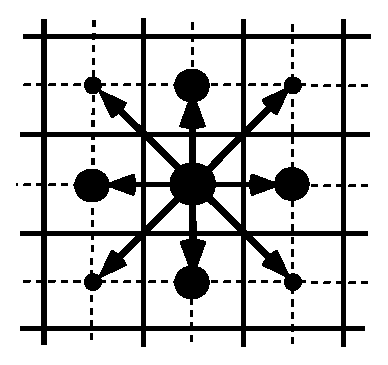
\includegraphics[width=0.66\textwidth]{LDF_ZDF1}
  \caption{Averaging procedure for isopycnal slope computation}
  \label{fig:LDF_ZDF1}
\end{figure}

%There are three additional questions about the slope calculation.
%First the expression for the rotation tensor has been obtain assuming the "small slope" approximation, so a bound has to be imposed on slopes.
%Second, numerical stability issues also require a bound on slopes.
%Third, the question of boundary condition specified on slopes...

%from griffies: chapter 13.1....

% In addition and also for numerical stability reasons \citep{cox_OM87, griffies_bk04},
% the slopes are bounded by $1/100$ everywhere. This limit is decreasing linearly
% to zero fom $70$ meters depth and the surface (the fact that the eddies "feel" the
% surface motivates this flattening of isopycnals near the surface).

For numerical stability reasons \citep{cox_OM87, griffies_bk04}, the slopes must also be bounded by
the namelist scalar \np{rn_slpmax}{rn\_slpmax} (usually $1/100$) everywhere.
This constraint is applied in a piecewise linear fashion, increasing from zero at the surface to
$1/100$ at $70$ metres and thereafter decreasing to zero at the bottom of the ocean
(the fact that the eddies "feel" the surface motivates this flattening of isopycnals near the surface).
\colorbox{yellow}{The way slopes are tapered has be checked. Not sure that this is still what is actually done.}

\begin{figure}[!ht]
  \centering
  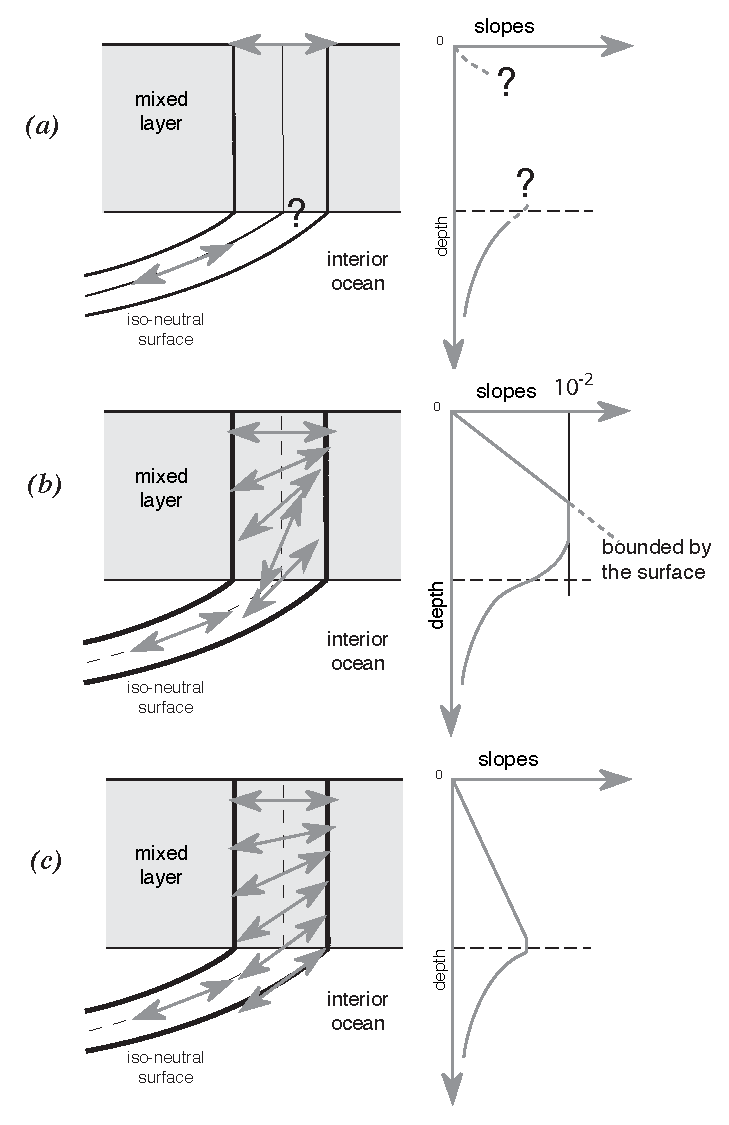
\includegraphics[width=0.66\textwidth]{LDF_eiv_slp}
  \caption[Vertical profile of the slope used for lateral mixing in the mixed layer]{
    Vertical profile of the slope used for lateral mixing in the mixed layer:
    \textit{(a)} in the real ocean the slope is the iso-neutral slope in the ocean interior,
    which has to be adjusted at the surface boundary
    \ie\ it must tend to zero at the surface since there is no mixing across the air-sea interface:
    wall boundary condition).
    Nevertheless,
    the profile between the surface zero value and the interior iso-neutral one is unknown,
    and especially the value at the base of the mixed layer;
    \textit{(b)} profile of slope using a linear tapering of the slope near the surface and
    imposing a maximum slope of 1/100;
    \textit{(c)} profile of slope actually used in \NEMO:
    a linear decrease of the slope from zero at the surface to
    its ocean interior value computed just below the mixed layer.
    Note the huge change in the slope at the base of the mixed layer between
    \textit{(b)} and \textit{(c)}.}
  \label{fig:LDF_eiv_slp}
\end{figure}

\colorbox{yellow}{add here a discussion about the flattening of the slopes, vs tapering the coefficient.}

%% =================================================================================================
\subsection{Slopes for momentum iso-neutral mixing}

The iso-neutral diffusion operator on momentum is the same as the one used on tracers but
applied to each component of the velocity separately
(see \autoref{eq:DYN_ldf_iso} in section~\autoref{subsec:DYN_ldf_iso}).
The slopes between the surface along which the diffusion operator acts and the surface of computation
($z$- or $s$-surfaces) are defined at $T$-, $f$-, and \textit{uw}- points for the $u$-component, and $T$-, $f$- and
\textit{vw}- points for the $v$-component.
They are computed from the slopes used for tracer diffusion,
\ie\ \autoref{eq:LDF_slp_geo} and \autoref{eq:LDF_slp_iso}:

\[
  % \label{eq:LDF_slp_dyn}
  \begin{aligned}
    &r_{1t}\ \ = \overline{r_{1u}}^{\,i}       &&&    r_{1f}\ \ &= \overline{r_{1u}}^{\,i+1/2} \\
    &r_{2f} \ \ = \overline{r_{2v}}^{\,j+1/2} &&& 	r_{2t}\ &= \overline{r_{2v}}^{\,j} \\
    &r_{1uw}  = \overline{r_{1w}}^{\,i+1/2} &&\ \ \text{and} \ \ &   r_{1vw}&= \overline{r_{1w}}^{\,j+1/2} \\
    &r_{2uw}= \overline{r_{2w}}^{\,j+1/2} &&&         r_{2vw}&= \overline{r_{2w}}^{\,j+1/2}\\
  \end{aligned}
\]

The major issue remaining is in the specification of the boundary conditions.
The same boundary conditions are chosen as those used for lateral diffusion along model level surfaces,
\ie\ using the shear computed along the model levels and with no additional friction at the ocean bottom
(see \autoref{sec:LBC_coast}).

%% =================================================================================================
\section[Lateral mixing coefficient (\forcode{nn_aht_ijk_t} \& \forcode{nn_ahm_ijk_t})]{Lateral mixing coefficient (\protect\np{nn_aht_ijk_t}{nn\_aht\_ijk\_t} \& \protect\np{nn_ahm_ijk_t}{nn\_ahm\_ijk\_t})}
\label{sec:LDF_coef}

The specification of the space variation of the coefficient is made in modules \mdl{ldftra} and \mdl{ldfdyn}.
The way the mixing coefficients are set in the reference version can be described as follows:

%% =================================================================================================
\subsection[Mixing coefficients read from file (\forcode{=-20, -30})]{ Mixing coefficients read from file (\protect\np[=-20, -30]{nn_aht_ijk_t}{nn\_aht\_ijk\_t} \& \protect\np[=-20, -30]{nn_ahm_ijk_t}{nn\_ahm\_ijk\_t})}

Mixing coefficients can be read from file if a particular geographical variation is needed. For example, in the ORCA2 global ocean model,
the laplacian viscosity operator uses $A^l$~= 4.10$^4$ m$^2$/s poleward of 20$^{\circ}$ north and south and
decreases linearly to $A^l$~= 2.10$^3$ m$^2$/s at the equator \citep{madec.delecluse.ea_JPO96, delecluse.madec_icol99}.
Similar modified horizontal variations can be found with the Antarctic or Arctic sub-domain options of ORCA2 and ORCA05.
The provided fields can either be 2d (\np[=-20]{nn_aht_ijk_t}{nn\_aht\_ijk\_t}, \np[=-20]{nn_ahm_ijk_t}{nn\_ahm\_ijk\_t}) or 3d (\np[=-30]{nn_aht_ijk_t}{nn\_aht\_ijk\_t},  \np[=-30]{nn_ahm_ijk_t}{nn\_ahm\_ijk\_t}). They must be given at U, V points for tracers and T, F points for momentum (see \autoref{tab:LDF_files}).

\begin{table}[htb]
  \centering
  \begin{tabular}{|l|l|l|l|}
    \hline
    Namelist parameter				            & Input filename	                             & dimensions	& variable names                      \\	\hline
    \np[=-20]{nn_ahm_ijk_t}{nn\_ahm\_ijk\_t}	    & \forcode{eddy_viscosity_2D.nc }            &     $(i,j)$	        & \forcode{ahmt_2d, ahmf_2d}  \\	\hline
    \np[=-20]{nn_aht_ijk_t}{nn\_aht\_ijk\_t}           & \forcode{eddy_diffusivity_2D.nc }           &     $(i,j)$	        & \forcode{ahtu_2d, ahtv_2d}    \\	\hline
    \np[=-30]{nn_ahm_ijk_t}{nn\_ahm\_ijk\_t} 	    & \forcode{eddy_viscosity_3D.nc }            &     $(i,j,k)$	        & \forcode{ahmt_3d, ahmf_3d}  \\	\hline
    \np[=-30]{nn_aht_ijk_t}{nn\_aht\_ijk\_t}	    & \forcode{eddy_diffusivity_3D.nc }           &     $(i,j,k)$	        & \forcode{ahtu_3d, ahtv_3d}    \\	\hline
  \end{tabular}
  \caption{Description of expected input files if mixing coefficients are read from NetCDF files}
  \label{tab:LDF_files}
\end{table}

%% =================================================================================================
\subsection[Constant mixing coefficients (\forcode{=0})]{ Constant mixing coefficients (\protect\np[=0]{nn_aht_ijk_t}{nn\_aht\_ijk\_t} \& \protect\np[=0]{nn_ahm_ijk_t}{nn\_ahm\_ijk\_t})}

If constant, mixing coefficients are set thanks to a velocity and a length scales ($U_{scl}$, $L_{scl}$) such that:

\begin{equation}
  \label{eq:LDF_constantah}
  A_o^l = \left\{
    \begin{aligned}
      & \frac{1}{2} U_{scl} L_{scl}  		     & \text{for laplacian operator } \\
      & \frac{1}{12} U_{scl} L_{scl}^3                    & \text{for bilaplacian operator }
    \end{aligned}
  \right.
\end{equation}

 $U_{scl}$ and $L_{scl}$ are given by the namelist parameters \np{rn_Ud}{rn\_Ud}, \np{rn_Uv}{rn\_Uv}, \np{rn_Ld}{rn\_Ld} and \np{rn_Lv}{rn\_Lv}.

%% =================================================================================================
\subsection[Vertically varying mixing coefficients (\forcode{=10})]{Vertically varying mixing coefficients (\protect\np[=10]{nn_aht_ijk_t}{nn\_aht\_ijk\_t} \& \protect\np[=10]{nn_ahm_ijk_t}{nn\_ahm\_ijk\_t})}

In the vertically varying case, a hyperbolic variation of the lateral mixing coefficient is introduced in which
the surface value is given by \autoref{eq:LDF_constantah}, the bottom value is 1/4 of the surface value,
and the transition takes place around z=500~m with a width of 200~m.
This profile is hard coded in module \mdl{ldfc1d\_c2d}, but can be easily modified by users.

%% =================================================================================================
\subsection[Mesh size dependent mixing coefficients (\forcode{=20})]{Mesh size dependent mixing coefficients (\protect\np[=20]{nn_aht_ijk_t}{nn\_aht\_ijk\_t} \& \protect\np[=20]{nn_ahm_ijk_t}{nn\_ahm\_ijk\_t})}

In that case, the horizontal variation of the eddy coefficient depends on the local mesh size and
the type of operator used:
\begin{equation}
  \label{eq:LDF_title}
  A_l = \left\{
    \begin{aligned}
      & \frac{1}{2} U_{scl}  \max(e_1,e_2)  			& \text{for laplacian operator } \\
      & \frac{1}{12} U_{scl}  \max(e_1,e_2)^{3}             & \text{for bilaplacian operator }
    \end{aligned}
  \right.
\end{equation}
where $U_{scl}$ is a user defined velocity scale (\np{rn_Ud}{rn\_Ud}, \np{rn_Uv}{rn\_Uv}).
This variation is intended to reflect the lesser need for subgrid scale eddy mixing where
the grid size is smaller in the domain.
It was introduced in the context of the DYNAMO modelling project \citep{willebrand.barnier.ea_PO01}.
Note that such a grid scale dependance of mixing coefficients significantly increases the range of stability of
model configurations presenting large changes in grid spacing such as global ocean models.
Indeed, in such a case, a constant mixing coefficient can lead to a blow up of the model due to
large coefficient compare to the smallest grid size (see \autoref{sec:TD_forward_imp}),
especially when using a bilaplacian operator.

\colorbox{yellow}{CASE \np{nn_aht_ijk_t}{nn\_aht\_ijk\_t} = 21 to be added}

%% =================================================================================================
\subsection[Mesh size and depth dependent mixing coefficients (\forcode{=30})]{Mesh size and depth dependent mixing coefficients (\protect\np[=30]{nn_aht_ijk_t}{nn\_aht\_ijk\_t} \& \protect\np[=30]{nn_ahm_ijk_t}{nn\_ahm\_ijk\_t})}

The 3D space variation of the mixing coefficient is simply the combination of the 1D and 2D cases above,
\ie\ a hyperbolic tangent variation with depth associated with a grid size dependence of
the magnitude of the coefficient.

%% =================================================================================================
\subsection[Velocity dependent mixing coefficients (\forcode{=31})]{Flow dependent mixing coefficients (\protect\np[=31]{nn_aht_ijk_t}{nn\_aht\_ijk\_t} \& \protect\np[=31]{nn_ahm_ijk_t}{nn\_ahm\_ijk\_t})}
In that case, the eddy coefficient is proportional to the local velocity magnitude so that the Reynolds number $Re =  \lvert U \rvert  e / A_l$ is constant (and here hardcoded to $12$):
\colorbox{yellow}{JC comment: The Reynolds is effectively set to 12 in the code for both operators but shouldn't it be 2 for Laplacian ?}

\begin{equation}
  \label{eq:LDF_flowah}
  A_l = \left\{
    \begin{aligned}
      & \frac{1}{12} \lvert U \rvert e  			& \text{for laplacian operator } \\
      & \frac{1}{12} \lvert U \rvert e^3 		        & \text{for bilaplacian operator }
    \end{aligned}
  \right.
\end{equation}

%% =================================================================================================
\subsection[Deformation rate dependent viscosities (\forcode{nn_ahm_ijk_t=32})]{Deformation rate dependent viscosities (\protect\np[=32]{nn_ahm_ijk_t}{nn\_ahm\_ijk\_t})}

This option refers to the \citep{smagorinsky_MW63} scheme which is here implemented for momentum only. Smagorinsky chose as a
characteristic time scale $T_{smag}$ the deformation rate and for the lengthscale $L_{smag}$ the maximum wavenumber possible on the horizontal grid, e.g.:

\begin{equation}
  \label{eq:LDF_smag1}
  \begin{split}
    T_{smag}^{-1} & = \sqrt{\left( \partial_x u - \partial_y v\right)^2 + \left( \partial_y u + \partial_x v\right)^2  } \\
    L_{smag} & = \frac{1}{\pi}\frac{e_1 e_2}{e_1 + e_2}
  \end{split}
\end{equation}

Introducing a user defined constant $C$ (given in the namelist as \np{rn_csmc}{rn\_csmc}), one can deduce the mixing coefficients as follows:

\begin{equation}
  \label{eq:LDF_smag2}
  A_{smag} = \left\{
    \begin{aligned}
      & C^2  T_{smag}^{-1}  L_{smag}^2			& \text{for laplacian operator } \\
      & \frac{C^2}{8} T_{smag}^{-1} L_{smag}^4     	& \text{for bilaplacian operator }
    \end{aligned}
  \right.
\end{equation}

For stability reasons, upper and lower limits are applied on the resulting coefficient (see \autoref{sec:TD_forward_imp}) so that:
\begin{equation}
  \label{eq:LDF_smag3}
    \begin{aligned}
      & C_{min} \frac{1}{2}   \lvert U \rvert  e    < A_{smag} < C_{max} \frac{e^2}{   8\rdt}                 & \text{for laplacian operator } \\
      & C_{min} \frac{1}{12} \lvert U \rvert  e^3 < A_{smag} < C_{max} \frac{e^4}{64 \rdt}                 & \text{for bilaplacian operator }
    \end{aligned}
\end{equation}

where $C_{min}$ and $C_{max}$ are adimensional namelist parameters given by \np{rn_minfac}{rn\_minfac} and \np{rn_maxfac}{rn\_maxfac} respectively.

%% =================================================================================================
\subsection{About space and time varying mixing coefficients}

The following points are relevant when the eddy coefficient varies spatially:

(1) the momentum diffusion operator acting along model level surfaces is written in terms of curl and
divergent components of the horizontal current (see \autoref{subsec:MB_ldf}).
Although the eddy coefficient could be set to different values in these two terms,
this option is not currently available.

(2) with an horizontally varying viscosity, the quadratic integral constraints on enstrophy and on the square of
the horizontal divergence for operators acting along model-surfaces are no longer satisfied
(\autoref{sec:INVARIANTS_dynldf_properties}).

%% =================================================================================================
\section[Eddy induced velocity (\forcode{ln_ldfeiv})]{Eddy induced velocity (\protect\np{ln_ldfeiv}{ln\_ldfeiv})}

\label{sec:LDF_eiv}

\begin{listing}
  \nlst{namtra_eiv}
  \caption{\forcode{&namtra_eiv}}
  \label{lst:namtra_eiv}
\end{listing}

%%gm  from Triad appendix  : to be incorporated....
\cmtgm{
  Values of iso-neutral diffusivity and GM coefficient are set as described in \autoref{sec:LDF_coef}.
  If none of the keys \key{traldf\_cNd}, N=1,2,3 is set (the default), spatially constant iso-neutral $A_l$ and
  GM diffusivity $A_e$ are directly set by \np{rn_aeih_0}{rn\_aeih\_0} and \np{rn_aeiv_0}{rn\_aeiv\_0}.
  If 2D-varying coefficients are set with \key{traldf\_c2d} then $A_l$ is reduced in proportion with horizontal
  scale factor according to \autoref{eq:title}
  \footnote{
    Except in global ORCA  $0.5^{\circ}$ runs with \key{traldf\_eiv},
    where $A_l$ is set like $A_e$ but with a minimum vale of $100\;\mathrm{m}^2\;\mathrm{s}^{-1}$
  }.
  In idealised setups with \key{traldf\_c2d}, $A_e$ is reduced similarly, but if \key{traldf\_eiv} is set in
  the global configurations with \key{traldf\_c2d}, a horizontally varying $A_e$ is instead set from
  the Held-Larichev parameterisation
  \footnote{
    In this case, $A_e$ at low latitudes $|\theta|<20^{\circ}$ is further reduced by a factor $|f/f_{20}|$,
    where $f_{20}$ is the value of $f$ at $20^{\circ}$~N
  } (\mdl{ldfeiv}) and \np{rn_aeiv_0}{rn\_aeiv\_0} is ignored unless it is zero.
}

When  \citet{gent.mcwilliams_JPO90} diffusion is used (\np[=.true.]{ln_ldfeiv}{ln\_ldfeiv}),
an eddy induced tracer advection term is added,
the formulation of which depends on the slopes of iso-neutral surfaces.
Contrary to the case of iso-neutral mixing, the slopes used here are referenced to the geopotential surfaces,
\ie\ \autoref{eq:LDF_slp_geo} is used in $z$-coordinates,
and the sum \autoref{eq:LDF_slp_geo} + \autoref{eq:LDF_slp_iso} in $s$-coordinates.

If isopycnal mixing is used in the standard way, \ie\ \np[=.false.]{ln_traldf_triad}{ln\_traldf\_triad}, the eddy induced velocity is given by:
\begin{equation}
  \label{eq:LDF_eiv}
  \begin{split}
    u^* & = \frac{1}{e_{2u}e_{3u}}\; \delta_k \left[e_{2u} \, A_{uw}^{eiv} \; \overline{r_{1w}}^{\,i+1/2} \right]\\
    v^* & = \frac{1}{e_{1u}e_{3v}}\; \delta_k \left[e_{1v} \, A_{vw}^{eiv} \; \overline{r_{2w}}^{\,j+1/2} \right]\\
    w^* & = \frac{1}{e_{1w}e_{2w}}\; \left\{ \delta_i \left[e_{2u} \, A_{uw}^{eiv} \; \overline{r_{1w}}^{\,i+1/2} \right] + \delta_j \left[e_{1v} \, A_{vw}^{eiv} \; \overline{r_{2w}}^{\,j+1/2} \right] \right\} \\
  \end{split}
\end{equation}
where $A^{eiv}$ is the eddy induced velocity coefficient whose value is set through \np{nn_aei_ijk_t}{nn\_aei\_ijk\_t} \nam{tra_eiv}{tra\_eiv} namelist parameter.
The three components of the eddy induced velocity are computed in \rou{ldf\_eiv\_trp} and
added to the eulerian velocity in \rou{tra\_adv} where tracer advection is performed.
This has been preferred to a separate computation of the advective trends associated with the eiv velocity,
since it allows us to take advantage of all the advection schemes offered for the tracers
(see \autoref{sec:TRA_adv}) and not just the $2^{nd}$ order advection scheme as in
previous releases of OPA \citep{madec.delecluse.ea_NPM98}.
This is particularly useful for passive tracers where \emph{positivity} of the advection scheme is of
paramount importance.

At the surface, lateral and bottom boundaries, the eddy induced velocity,
and thus the advective eddy fluxes of heat and salt, are set to zero.
The value of the eddy induced mixing coefficient and its space variation is controlled in a similar way as for lateral mixing coefficient described in the preceding subsection (\np{nn_aei_ijk_t}{nn\_aei\_ijk\_t}, \np{rn_Ue}{rn\_Ue}, \np{rn_Le}{rn\_Le} namelist parameters).
\colorbox{yellow}{CASE \np{nn_aei_ijk_t}{nn\_aei\_ijk\_t} = 21 to be added}

In case of setting \np[=.true.]{ln_traldf_triad}{ln\_traldf\_triad}, a skew form of the eddy induced advective fluxes is used, which is described in \autoref{apdx:TRIADS}.

%% =================================================================================================
\section[Mixed layer eddies (\forcode{ln_mle})]{Mixed layer eddies (\protect\np{ln_mle}{ln\_mle})}
\label{sec:LDF_mle}

\begin{listing}
  \nlst{namtra_mle}
  \caption{\forcode{&namtra_mle}}
  \label{lst:namtra_mle}
\end{listing}

If  \np[=.true.]{ln_mle}{ln\_mle} in \nam{tra_mle}{tra\_mle} namelist, a parameterization of the mixing due to unresolved mixed layer instabilities is activated (\citet{foxkemper.ferrari_JPO08}). Additional transport is computed in \rou{ldf\_mle\_trp} and added to the eulerian transport in \rou{tra\_adv} as done for eddy induced advection.

\colorbox{yellow}{TBC}

\subinc{
\clearpage

%% Bibliography
\phantomsection
\addcontentsline{toc}{chapter}{Bibliography}
\lohead{Bibliography} \rehead{Bibliography}
\bibliography{../main/bibliography}

\clearpage

%% Indexes
\phantomsection
\addcontentsline{toc}{chapter}{Indexes}
\lohead{Indexes} \rehead{Indexes}
\printindex[blocks]
\printindex[keys]
\printindex[modules]
\printindex[parameters]
\printindex[subroutines]
}

\end{document}
